% This is samplepaper.tex, a sample chapter demonstrating the
% LLNCS macro package for Springer Computer Science proceedings;
% Version 2.20 of 2017/10/04
%
\documentclass[runningheads]{llncs}
%
\usepackage{float}
\usepackage{graphicx}
% Used for displaying a sample figure. If possible, figure files should
% be included in EPS format.
\usepackage{color}
\usepackage{hyperref}
% If you use the hyperref package, please uncomment the following line
% to display URLs in blue roman font according to Springer's eBook style:
\renewcommand\UrlFont{\color{blue}\rmfamily}
\def\sectionautorefname{Section}
\def\subsectionautorefname{Subsection}

\begin{document}
%
\title{Analysis of and Mitigation Strategies for \\Real World ICS Security Incidents}
%
%\titlerunning{Abbreviated paper title}
% If the paper title is too long for the running head, you can set
% an abbreviated paper title here
%
\author{Nico Fechtner}
%
\authorrunning{N. Fechtner}
% First names are abbreviated in the running head.
% If there are more than two authors, 'et al.' is used.
%
\institute{Technical University of Munich \& \\Fraunhofer Institute for Applied and Integrated Security\\
\href{mailto:nico.fechtner@tum.de}{nico.fechtner@tum.de}}
%
\maketitle              % typeset the header of the contribution
%
\begin{abstract}
% The abstract should briefly summarize the contents of the paper in
% 150--200 words.
% The goal is to communicate: Background/motivation/context, Aim/objective(s)/problem statement, Approach/method(s)/procedure(s), Results, Conclusion(s)/implications.
More and more Industrial Control Systems (ICS) are getting connected to enterprise IT networks and the internet.
Due to this, the attack surface of these systems increases, which led to a high number of real world ICS security incidents over the last years.
It is therefore crucial to analyze and learn from past incidents to avoid common mistakes and to develop efficient detection and mitigation strategies that help to prevent future incidents.
To support this process, this paper proposes a systematic comparative overview of historic ICS security incidents and an in-depth analysis of the Triton incident.
Key findings include the following.
Untargeted ransomware attacks as well as targeted state-sponsored operations both present prevalent threats to the ICS landscape.
Adversaries often use techniques like spearphishing, zero-day exploits, sophisticated obfuscation, and evasion techniques, and living off the land tools to extract data and cause disruption.
Suitable defense strategies include increasing the security awareness of employees, strictly separating the ICS network from the enterprise IT network, and establishing a reliable backup strategy.

\keywords{ICS Security \and ICS Attacks \and Threat Actors \and Triton.}
\end{abstract}
%
%
%

\section{Introduction}
% The introduction supplies sufficient background information for the reader to understand and evaluate the work you did. Assume the reader is a generic computer science student, knowledgeable and acquainted with all basic computer science concepts. The introduction should also include a description of the problem you want to solve, your research questions, and an outline for the remainder of your paper. The goal is to: Indicate the field of the work, why this field is important, and what has already been done (with proper citations), Outline the purpose of your paper and announce your research questions, Avoid: repeating the abstract; providing unnecessary background information.
% While Information Technology (IT) refers to software and hardware that generate data for enterprise use, Operational Technology (OT) describes software and hardware able to detect or cause a physical event in an industrial environment.
% % ICS
% The most prominent subcategory of OT are Industrial Control Systems (ICS).
% They are used in a wide variety of industries such as food and agriculture, energy, water, transportation, chemical, nuclear power, pharmaceutical, and discrete manufacturing \cite{stouffer.2011}.\\
% OT Security <-> IT Security: very recent trend, first incidents
Industrial Control Systems (ICS) are used in a wide variety of industries such as food and agriculture, energy, water, transportation, chemical, nuclear power, pharmaceutical, and discrete manufacturing \cite{stouffer.2011}.
Initially, they were not connected to the internet and strictly separated from enterprise IT networks.
Due to this isolation, it was hard, if not impossible, for adversaries to remotely attack ICS, which is why until recently security was not a big concern to companies running ICS.
% Instead, they traditionally focus on the safety, continuity, and efficiency of their systems.
However, the attack surface of many ICS changed within the last two decades since they got connected to traditional IT networks and the internet---sometimes intentionally, sometimes by mistake.
Inevitably, this led to an ongoing series of ICS security incidents.\\
% Problem: No overview; Contribution: Overview
While more and more of those incidents are reported, it is business-critical to develop suitable detection and mitigation strategies.
An essential baseline in this process is analyzing and learning from past incidents.
This is crucial to avoid common mistakes and to effectively prevent future incidents.
To support this process, this paper proposes a systematic comparative overview of historic ICS security incidents focusing on various parameters including targets, threat actors, attack techniques, goals and impacts, dwell times, operator reactions, and detection and mitigation strategies.
% Benefits of an overview: Helps to identify patterns and to prevent future incidents (?)
The overview aims at identifying common attack patterns that could be used to prevent future attacks.
To the best of the author's knowledge, such an overview has not yet been published.\\
% Triton
Additionally, the Triton incident of 2017 is analyzed in detail to showcase how attackers perform sophisticated ICS attacks and which detection and mitigation strategies can be derived from their methodologies.\\
% The incident was chosen due to its potential life-threatening impact and the novel attack approach targeting Safety Instrumented Systems (SIS).\\

% Outline
The remainder of the paper is structured as follows.
\autoref{section:related-work} provides an overview of related work in the area of ICS incidents, which is used as the basis of the comparative overview that is provided in \autoref{section:overview}.
Exemplary the Triton incident is analyzed in detail in \autoref{section:triton}.
\autoref{section:conclusion} concludes the paper by summarizing key findings and suggesting directions for future work.

\section{Related Work}
\label{section:related-work}
% In this section, you provide an overview of papers written by other scientists that have covered a problem similar to yours. You can find related work in web search engines and scientific literature databases. Some of the most prominent ones in the field of computer science are: Google Scholar, Scopus, ACM Digital Library, IEEE Xplore, Lecture Notes in Computer Science.
There are four main types of publicly available sources that provide information on ICS security incidents.
% Enumerations: RISI Database, ICS-CERT Alerts from the US Government,
First, there are incident enumerations like the Risi Database\footnote{\url{https://www.risidata.com/Database}} and the ICS-CERT Alerts\footnote{\url{https://www.us-cert.gov/ics/alerts}}.
% On the one hand, the fact that those repositories aim to aggregate all observed ICS incidents from around the world makes them useful for getting a high-level overview of the current threat landscape.
% On the other hand, however, they only provide basic information about the incidents and do not analyze them in detail.
% Reports from Companies in the field: Dragos Threat Report, CyberX Global IoT/ICS Risk Report,...
Second, ICS security companies like Dragos \cite{dragos.19} and CyberX \cite{cyberx.19} publish yearly ICS threat reports discussing relevant incidents.
% Those reports are neither complete with regards to the incidents they cover nor do they provide in-depth analyses of the covered attacks.
% However, they highlight important trends in the threat landscape throughout the years.
Third, dedicated scientific papers are focusing on single ICS incidents like the attacks targeting the Ukraine power grid \cite{eisac.16} or the Triton malware \cite{pinto.18}.
% Those papers usually cover single incidents in-depth and help in understanding how exactly the adversaries operated.
Fourth, there are numerous blog posts, press releases, and conference talks covering ICS incidents.
In addition, there is the MITRE ATT\&CK ICS database\footnote{\url{https://collaborate.mitre.org/attackics/index.php}} which includes information on tactics, techniques, and software used by threat groups to perform ICS attacks.
Furthermore, there is a paper proposing an overview of historical ICS security incidents \cite{hemsley.18}.
However, it is slightly dated and, more importantly, does not compare the different incidents systematically.
All of the above-mentioned sources are taken into account to achieve exactly this in the upcoming section.

% Other papers covering the big incidents: Ukraine, Triton,...
% IT incidents overview
\section{Comparative Overview of ICS Security Incidents}
\label{section:overview}
From the literature and resources stated in \autoref{section:related-work}, a total of 27 ICS security incidents were extracted.
Those are the basis of the following analysis and can be found in \autoref{tab:incidents}.
Note that due to incidents not being reported, the high number of incidents that are reported and new incidents occurring steadily, this table is inherently incomplete, but rather tries to focus on the most prevalent attacks launched until February 2020.
The following subsections provide a comparative overview of these incidents.
Each subsection aims to compare the incidents with regards to specific attributes, e.g. the involved threat actors or the utilized attack techniques.
% (
% Most subsections contain both quantitative as well as qualitative statements.
% Please keep in mind, though, that the quantitative numbers are solely intended to highlight important trends and that the according values might contains inaccuracies.
% This is due to the fact that often specific information about incidents is unknown or not known for sure.
% )
\begin{table}[h]
	\centering
    \begin{tabular}{|l|l|l|l|l|}
    \hline
    \textbf{Incident}               & \multicolumn{1}{l|}{\textbf{Impact}} & \multicolumn{1}{l|}{\textbf{Targeted}} & \multicolumn{1}{l|}{\textbf{Region}} & \textbf{Sector} \\ \hline
    Maroochy Water                  & 2000                                       & Yes                                    & Australia                                    & (Waste)water                         \\
    Conficker                       & 2008                                       & No                                     & Multiple                              & Multiple                             \\
    Stuxnet                         & 2010                                       & Yes                                    & Iran                                         & Nuklear Power                        \\
    NightDragon                     & 2010                                       & Yes                                    & Global                                       & Multiple                             \\
    Duqu                            & 2011                                       & Yes                                    & Multiple                                     & Multiple                            \\
    Gas Pipeline Intrusion Campaign & 2011                                       & Yes                                    & Unknown                                            & Energy                               \\
    Shamoon                         & 2012                                       & Yes                                    & Middle East                                  & Energy                               \\
    Flame/sKyWIper                  & 2012                                       & No                                     & Middle East                                  & Unknown                                    \\
    Gauss                           & 2012                                       & Yes                                    & Middle East                                  & Unknown                                    \\
    Red October                     & 2013                                       & Yes                                    & Multiple                                     & Gov / Research                       \\
    Target Store's HVAC             & 2013                                       & Yes                                    & US                                           & Retail                               \\
    New York Dam                    & 2013                                       & Yes                                    & US                                           & Water                               \\
    Havex/Backdoor.Oldrea           & 2013                                       & Yes                                    & US/Europe                                    & Multiple                             \\
    German Steel Mill               & 2014                                       & Yes                                    & Germany                                      & Manufacturing                    \\
    BlackEnergy(3)                  & 2015                                       & Yes                                    & Ukraine                                      & Energy                               \\
    Industroyer/CRASHOVERRIDE       & 2016                                       & Yes                                    & Ukraine                                      & Energy                               \\
    “Kemuri” water company          & 2016                                       & Yes                                    & US                                       & Water                                \\
    Op Ghoul                        & 2016                                       & Yes                                    & Multiple                                     & Multiple                             \\
    WannaCry                        & 2017                                       & No                                     & Multiple                                     & Multiple                             \\
    NotPetya                        & 2017                                       & Yes                                    & Ukraine                              & Multiple                             \\
    BitPaymer                       & 2017                                       & Yes                                    & Multiple                                     & Multiple                             \\
    Dragonfly 2.0                   & 2017                                       & Yes                                    & Unknown                                            & Energy                               \\
    Triton/Trisis/Hatman            & 2017                                       & Yes                                    & Saudi Arabia                                 & Chemical                  \\
    StoneDrill                      & 2017                                       & Yes                                    & Saudi Arabia                                 & Unknown                                    \\
    Shamoon 3                       & 2018                                       & Yes                                    & Multiple                                     & Multiple                             \\
    LockerGoga                      & 2019                                       & Yes                                    & Multiple                                     & Multiple                             \\
    Maze/ChaCha                     & 2019                                       & No                                     & Multiple                                     & Multiple\\
    \hline
    \end{tabular}
    \medskip\medskip
    \caption{ICS incidents considered in the comparative analysis ordered by the time of their first impact.}
    \label{tab:incidents}
    \end{table}


\subsection{Targets}
\label{subsection:overview-targets}
% Targeted vs. Untargeted
When analyzing the entities affected by ICS security incidents there are two fundamentally different kinds of attacks that have to be considered separately.
On the one hand, there are targeted attacks against unique entities.
Making up roughly 85\% of the analyzed incidents, targeted attacks seem to present a diverse threat landscape to ICS and are therefore analyzed in detail below.
On the other hand, there are untargeted attacks.
Here, the threat actors are not interested in the specific entities that will be affected by the attack, but rather aim for as many incidents as possible.
Often this is achieved by a self-replicating component within the malware used for the attacks.
While only four of the analyzed incidents fall into this category, they still pose a significant threat to ICS.
Interesting to see is that the malware used for untargeted attacks usually is not tailored specifically for ICS environments, but rather targets common operating systems like Microsoft Windows and enterprise networks in general.
Many instances of untargeted attacks fall in the category of ransomware.
For example, the popular WannaCry ransomware spread not only to desktop computers around the world but also infected a series of ICS workstations e.g. at a Taiwanese manufacturing plant leading to outages due to encrypted hard drives \cite{skybox.18}.
This kind of incidental infections of ICS systems with malware originally intended for enterprise networks are becoming more and more of a threat in recent years \cite{dragos.19}, \cite{cyberx.19}, \cite{zimba.18}.\\
% Untargeted
Since untargeted attacks are not aimed at specific entities but often solely intend to infect as many systems as possible, e.g. with self-replicating components, there is in general no pattern observable in terms of the geographical location or the economic sector of the affected parties.
Targeted attacks, however, can be analyzed for such patterns.\\
% Country
When it comes to the geographical location of ICS attack victims, the most affected regions seem to be Europe and the Middle East.
Companies located in Europe are targeted by about 37\% of the analyzed attacks.
The country affected the most until now is Ukraine falling victim to multiple attacks targeting its power grid.
The Middle East is being targeted by about 33\% of the analyzed attacks.
% Especially companies located in Saudi Arabia often fall victim to attacks.
% Probably the most well-known incident taking place there was Triton, which targeted a Saudi Arabian petrochemical plant and is covered in depth by \autoref{section:triton}.
In about 19\% of the analyzed incidents, the US were amongst the victims.
Note that while being home to important global threat actors as discussed in \autoref{subsection:overview-actors}, neither Russia nor China nor North Korea report a lot of ICS incidents against entities located in their countries.
% However, this does not necessarily mean that no ICS incidents occur in these countries, but it could also be the case that incidents are just not as liberally published as by other countries.
% Especially China and North Korea are known for withholding most of the cyber attacks taking place in their country [citation].
\\
% Sector (+ private/public)
When it comes to the economic sectors falling victim to targeted ICS attacks, the most affected one is the energy sector being targeted in at least 37\% of the analyzed targeted attacks.
Often, those operations include attacks against power grids like the attacks taking place in 2014 and 2015 in Ukraine.
Other examples of targeted entities within the energy sector include oil and gas pipelines as well as refineries.
The remaining victims of ICS attacks are spread across a wide variety of other economic sectors including manufacturing, water, petrochemical, governmental organizations, and transportation.

\subsection{Threat Actors}
\label{subsection:overview-actors}
% General
In total, at least 16 specific threat actors were involved in the analyzed ICS incidents according to the current state of research.
% (
% Note, that there are often multiple names for a single threat group that originate from different ICS security agencies and companies \cite{thaicert.19} and can be used interchangeably.
% This paper tries to use to the most commonly used names regardless of which entity coined them.\\
% )
% Problem of Attribution
When it comes to the threat actors responsible for ICS attacks there is the fundamental issue of attribution.
Usually, threat actors want to stay anonymous and do not confess performed attacks. % Counterexample?
Therefore, there are often only conjectures about the threat actors involved in certain attacks.
In line with that, 37\% of the analyzed attacks cannot be associated with a specific threat actor.
% Where are Threat actors located?
Furthermore, it is often difficult to locate threat actors geographically, since they usually apply various techniques to hide their physical location \cite{huang.18}.
With regards to the analyzed incidents, 33\% of the threat groups cannot be associated with a specific country.
It can be said, however, that 30\% of all analyzed attacks are assumed to originate from Russia and 22\% from the Middle East, thereof 67\% from Iran.
Other countries being home to important threat groups are China, the US, and North Korea.
% Which are the most important threat actors?
The most active threat actors according to the sample of incidents taken into account here are Energetic Bear from Russia, being involved in at least 15\% of all attacks, and APT33 from Iran, being involved in at least 11\% of all attacks.
% Collaboration
Interesting to note is that some threat groups primarily act on their own while others tend to collaborate with others.
For example, APT33 often collaborates with other Iranian threat groups, whereas Energetic Bear mostly acts on its own.
% Team Size
When it comes to the team size, only one threat actor corresponds to a single person---Vitak Boden in the Maroochy Water incident.
% This person, Vitak Boden, performed what can be considered one of the first ICS attacks ever.
% To take revenge on a wastewater facility where he was rejected when applying for a job, he manipulated the sewage pumping stations via a radio frequency transmitter, which lead to millions of gallons of untreated sewage water being released into waterways and local parks \cite{hemsley.18}.
Since this incident in the year 2000, ICS attacks got a lot more sophisticated which is why the team size of threat groups continues to grow.\\
% Who is behind threat groups? Nation State Actors?
At least 59\% of the analyzed attacks are considered to be performed by government-funded threat actors.
On the one hand, targeted ICS attacks require a large amount of knowledge and resources to which often only state-sponsored groups have access to.
On the other hand, governments can profit in various ways from ICS attacks against foreign countries, be it through industrial espionage, by making critical facilities and infrastructures unavailable or even by targeting human lives.
ICS attacks are therefore sometimes even considered an act of war \cite{lindsey.19}. % further research.

\subsection{Attack Techniques}
\label{subsection:overview-techniques}
% ICS cyber kill chain
An established model to characterize ICS attacks is the ICS Cyber Kill Chain depicted in \autoref{fig:CyberKillChain}.
It is comprised of two stages.
In stage one, IT intrusion preparation and execution happens, i.e. the attacker compromises the IT network and positions herself in the ICS network.
This stage can be completed without specific knowledge about ICS technologies or protocols.
In stage two, ICS attack development and execution are performed, e.g. an attack targeting certain actuators---for example, water pumps---is developed, tested, and executed.\\
When it comes to the initial access in stage one of the ICS Cyber Kill Chain, two attack techniques seem to be most popular among the analyzed incidents.
The first one is spearphishing, which was reportedly performed in at least 26\% of the attacks.
The second one is the utilization of zero-day exploits, which was observed in at least 11\% of the attacks.
When inside the victims' IT network, attackers often use common software.
For example, in at least 11\% of the cases, Mimikatz was used for credential capturing.
Popular exploitation frameworks like Metasploit and Cobalt Strike are frequently used, too.
More recent trends are the use of sophisticated obfuscation and evasion techniques and \textit{living off the land} tools---like PowerShell or PsExec---to avoid being detected by Intrusion Detection Systems (IDS).
\begin{figure}[H]
    \centering
    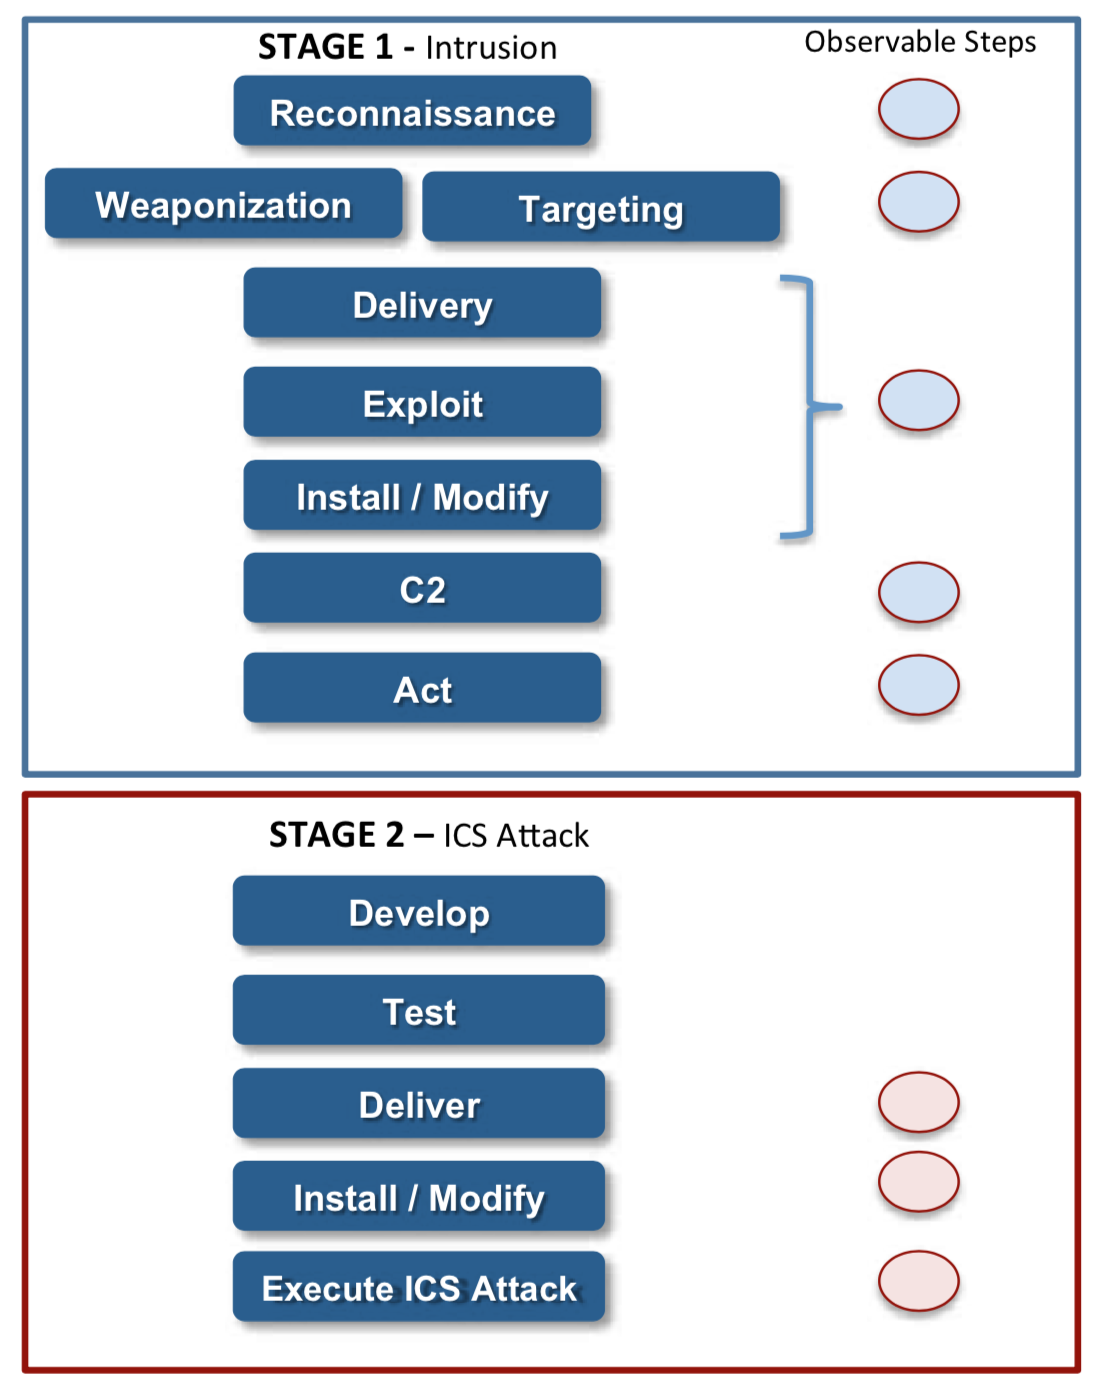
\includegraphics[width=8cm]{figures/ICSCyberKillChain.png}
    \caption{ICS Cyber Kill Chain as introduced by the SANS institute, from \cite{assante.15}.}
    \label{fig:CyberKillChain}
\end{figure}\noindent
% Untargeted Attacks
Since untargeted attacks usually rely on ransom- or wiperware, they do not go beyond stage one of the ICS Cyber Kill Chain.
% Targeted Attacks
Targeted attacks, however, aim more and more often to exploit specific ICS environments, which requires the attackers to first gain access to the ICS network.
One possible way to pivot is lateral movement via Windows authentication services.
% Stage 2: ICS Attack
Once in the ICS network, a multitude of different exploit strategies has been reported.
Most adversaries attack ICS components like Programmable Logic Controllers (PLCs) or Safety Instrumented Systems (SIS) to modify their behavior or to make them fail altogether.
Doing so, they are often able to control actuators like water pumps, fake the values of sensors, or turn off the power supply.
To make disaster recovery harder, attackers often wipe Human-Machine Interfaces (HMIs), too.
% Special Case: Target Store's HVAC
While according to the ICS Cyber Kill Chain stage one typically has to take place before stage two, there is an example where the attack was performed the other way around.
In 2013, an unknown attacker stole login credentials of a third-party heating, ventilation, and air conditioning (HVAC) contractor of US Target Stores.
From the ICS network, the adversary then pivoted into the IT network to install credit card stealing software. \cite{hemsley.18}\\
% Scalability of the attack: Trend goes to scalable frameworks?
One important trend in addition to the techniques described above is the trend away from manual attacks specifically tailored for a single victim towards more victim-agnostic ICS attack frameworks enabling scalable attacks.
A case in point are the attacks on the Ukraine power grid.
The first attack in 2015 was exclusively manual and the effort put into it could not be directly utilized for attacks against other energy infrastructures.
One year later, however, there was a second attack targeting the power grid, but this time the adversaries had developed a framework, which in theory allows them to scale their attack to a multitude of different victims with a relatively small effort. \cite{greenberg.17}

\subsection{Attack Goals and Realized Impacts}
\label{subsection:overview-goals}
% Common goals
The most common goal of adversaries is to extract data from the victim's systems. 37\% of all analyzed attacks were designed to achieve exactly this.
Other goals often pursued by attackers are to cause disruption (22\%), to provoke a ransom payment (15\%), and to cause physical damage (11\%).\\
% Underlying motivations (state actors)
When it comes to the underlying motivations of attackers, three distinct ones seem to dominate.
First, attackers often strive for monetary gain.
This motivates ransomware attacks like WannaCry or LockerGoga as well as information stealing with the goal of selling the data to the highest bidder.
Second, some adversaries are interested in the data they steal themself and do not intend to sell them.
This motivates ICS espionage operations like StoneDrill were Iranian threat groups gathered intelligence about Saudi Arabian ICS environments.
Third, there are threat actors that intend to disrupt the regular operation of ICS by causing outages or even physical damage.
The latter was e.g. the case in the famous Stuxnet incident in 2010 where the US and Israelian government attacked nuclear enrichment facilities of Iran to sabotage the possible development of nuclear weapons.
Untargeted attacks falling into this category are typically related to wiperware which erases or encrypts hard drives without a subsequent ransom demand.\\
% How often were they successful
In total, a minimum of 85\% of the attacks are considered to be at least partly successful in achieving their goals with regards to some of their victims.
% Impacts, when successful
Typical impacts include information loss, financial loss---via physical damage, ransom payment or costly recovery processes---and environmental damages.
Fortunately, until to date, there are no ICS incidents known that killed humans.\\
% If not successful, why?
One incident considered to be unsuccessful is the well-known Triton attack, which failed for reasons not fully understood up until today.
\autoref{section:triton} provides a detailed analysis of the incident and its impacts.
Furthermore, untargeted attacks often partly fail to achieve their goal since a lot of companies can restore operations without a long outage or paying a ransom thanks to sufficient backup strategies.

\subsection{Dwell Times and Reactions}
\label{subsection:overview-reactions}
% Dwell times
Dwell time describes how long an adversary is in a system before the actual attack payload is executed.
% While sometimes it is possible to give an accurate estimation for this number thanks to digital forensics after an incident, keep in mind that, in general, this is a non-trivial task and potentially leads to inaccuracies.
% A rough trend, however, can be detected when analyzing important ICS incidents.
% Untargeted: often days
In the context of untargeted attacks, the dwell time usually is a matter of days, while when speaking about targeted attacks, it typically ranges from multiple months, e.g. in the attacks targeting the Ukraine power grid and the Triton incident, to multiple years.
The latter is considered to be the case, for example, when considering the Red October espionage campaign against multiple countries initiated by a Russian threat actor.
% Targeted multiple months (Industroyer, Blackenergy, Triton) to multiple years (Red October)
% Lots of time to detect the intrusion
It seems that with dwell times this long it should be possible for the ICS network operators to detect that something is wrong within their systems before the adversaries deliver the final payload.
% However: Time of Discovery medium BlackEnergy & Triton but most often late
Unfortunately, while this holds in theory, attacks are usually not detected in their early stages in practice.
There are some cases---BlackEnergy and Triton---where the administrators were able to detect that something is wrong before the actual attack payload was executed, but in most cases, the attack is only detected after the final exploit was already delivered.\\
% Typical Reactions (do they help?)
% Untargeted attacks: Pay ransom (via insurance) or restore via backup (maybe buy new hard drives <-> Shamoon)
When it comes to reacting to an untargeted attack, there is sometimes the option to pay a ransom to get the hard drives decrypted again by the adversary.
While this should be avoided, since there is no certainty that the attackers will indeed decrypt the hard drives as promised, there are still cases known were the ransom was paid.
Often companies have dedicated insurances that cover such ransom demands under certain circumstances.
The typical response to a destructive untargeted attack, however, is to restore operations from backups.
% Targeted attacks: When medium usually shutdown like Triton
% When late digital forensics
In the case of targeted attacks, when operators suspect that an intrusion has happened, they often shut down the ICS to prevent further breaches, physical damage, and threats to human lives.
This happened, e.g. in the Triton incident.
When the final payload was already delivered by the adversaries, however, often the only thing left to do is to start recovery processes that aim to restore operations and typically also include digital forensics to analyze how the incident could have happened, e.g. how the ICS network could be breached, in the first place.
% As a result of the Shamoon attack, however, thousands of hard drives were destroyed irretrievably such that the affected company had to quickly buy large amounts of hard drives, which lead to a world-wide shortage of those.

\subsection{Detection and Mitigation Strategies}
\label{subsection:overview-mitigation}
% Mitigation against untargeted ransom- & wiperware
After comparatively analyzing 27 ICS incidents a multitude of potential detection and mitigation strategies can be identified which can be leveraged to defend ICS against future threats.\\
% Detection
% Asset Inventory
To be able to detect ongoing ICS attacks, the first fundamental resource is an up-to-date asset inventory.
Only with that, possibly dangerous network or host activity can be detected.
% Anomaly/Incident Detection System
Such detection is usually offered by IDS that lookout, e.g. on network tabs or SPAN ports, for anomalies in the network traffic.
Compared to traditional IT networks, this is a quite promising approach, since---in contrast to IT networks---the expected network traffic does not vary much such that false positives can be relatively easy tuned to a minimum.
% Threat Hunting
A more active approach to IDS is threat hunting where security specialists try to identify adversaries that already reside inside the victims' network.\\
% Mitigation
When it comes to suitable mitigation strategies, the first line of defense to strengthen are the humans operating ICS.
% Security Awareness
As stated in \autoref{subsection:overview-techniques}, many adversaries use social engineering for gaining an initial foothold in the victim's network.
The risk of successful phishing compromises can e.g. be reduced by security awareness workshops.
% Vulnerability Management Software
More on the technical side of things are vulnerability management solutions.
In ICS environments, it is often not that easy to patch hosts, since this could mean downtime and therefore revenue loss.
However, it is crucial to at least know which hosts have known vulnerabilities.
Even if a patch might not be possible, one could e.g. at least harden the network segmentation around the vulnerable hosts to make a compromise less likely.
% Firewalls
Inspired by traditional IT networks, firewalls are becoming more and more popular in ICS environments, too.
They are especially critical in overlapping parts of the IT and ICS networks.
% Backups
Last but not least, it is essential to have a solid backup strategy that allows for restoring operations fast and reliable, e.g. in the case of a ransom- or wiperware attack.

\section{Detailed Analysis of the Triton Attack}
\label{section:triton}
While the previous section conducted a comparative overview of the most prevalent ICS security incidents to highlight general trends, this section focusses on a specific attack to detail how insight gained from such an analysis can be used to prepare for future attacks.
Exemplary, the Triton attack targeting a Saudi Arabian petrochemical plant in 2017 is analyzed.
The incident---also known as Trisis \cite{dragos.17} and HatMan\footnote{\url{https://www.us-cert.gov/ics/MAR-17-352-01-HatMan—Safety-System-Targeted-Malware}}---is chosen as an example since it is considered to be of significant importance to the ICS community \cite{dragos.17}.
First and foremost it was the first attack targeting SIS and therefore potentially threatening human lives.
Additionally, the attack was highly sophisticated, and even when it was eventually detected by the plant operators, they were not able to stop it immediately.
% Outline?
\subsection{Attack and Response Strategies}
\label{subsection:triton-attack-response}
% Stage 1
% As described in \autoref{subsection:overview-techniques}, an ICS attack usually is comprised of the two stages of the ICS Cyber Kill Chain.
When it comes to Triton, the details of stage one of the ICS Cyber Kill Chain are still unclear.
It seems that the IT network of the Petro Rabigh oil refinery got breached already in 2014, however, the exact techniques used for the initial access and the movement into the ICS network are not unambiguously known.
It is suspected, however, that the initial access happened via a spearphishing attack \cite{nohe.19}.
\\
% Stage 2: Triton malware
Stage two of the ICS Cyber Kill Chain began shortly after the initial breach of the IT network when the attackers managed to access the Triconex SIS from Schneider Electric---therefore the name Triton or Trisis.
% Background: SIS
SIS are an integral part of ICS in that their sole purpose is to maintain safe operations should failures of other hard- or software occur.
They should prevent catastrophic incidents like explosions or fire and protect human lives \cite{pinto.18}.
It is therefore crucial that this last line of automated safety defense operates correctly.
% The functionality of an SIS can be broken down as follows.
The inputs for an SIS are an array of sensors measuring physical values e.g. temperature, pressure, or rotation speed.
In real-time, the SIS analyzes these values and outputs a single decision: if it is safe to continue operation.
Should the SIS decide that there is an unsafe physical condition, suitable commands are sent to according actuators like water pumps, machine engines, or valves. \cite{dragos.17}\\
% E.g. if an SIS would detect a dangerously high temperature in a gas tank, the valves regulating the gas inflow would be closed. \cite{dragos.17} \\
% Attack method
To protect an SIS from unintended modification, there is a physical keyswitch controlling the mode of operation.
Under normal circumstances, this switch should be set to \textit{run}, which disables arbitrary changes to the logic of the SIS.
In the case of Petro Rabigh, however, the switch was set to \textit{program mode}, which allows for logic changes.
Why this was the case is not known, but it might very likely be the case that an engineer programming the SIS simply forgot to switch it back to \textit{run} mode.
In addition to these modes of operation, network connectivity to an SIS should, in theory, be extremely limited if existent at all.
In practice, for example, plant operators sometimes want to retrieve data from SIS to analyze them, which is why they allow for more network connectivity than needed for reasons of convenience.
This might have been the case at Petro Rabigh, too.
\cite{dragos.17}\\
After the adversaries had found out the exact type of SIS the plant was using, they left for about two years.
It may very well be the case that in this timespan they managed to acquire a physical copy of the same type of SIS and developed a targeted malware that came to be known as Triton.
After this timeframe, they returned to the oil refinery and installed the malware on the SIS.
The goal of the malware was to change the internal logic of the SIS, which could lead to severe consequences.
It could, for example, reprogram the SIS in a way such that it would not shut down the plant in the case of an emergency. \cite{lee.20}\\
% First outage
Indeed, shortly after the malware was installed, the SIS tripped and shut down the oil refinery.
However, this shutdown was not intended by the attackers.
It turned out that it was rather the consequence of a programming error on their side, which instead of rewriting the logic of the SIS brought it down entirely, which led to a shutdown of the whole plant.
% Response
The plant operators in charge at this point did not consider the SIS failure as being the result of a targetted ICS attack.
Instead, they thought it must be some error of the SIS itself.
So they contacted the SIS vendor and hired some investigators, however, none of them was an ICS security specialist.
In the end, they were not able to identify the root cause of the shutdown and considered it to be a one time error.
Eventually, they brought up the refinery again. \cite{lee.20}\\
% Attackers response
This meant that the adversaries got a second chance to attack.
Indeed, they were able to identify the bug, which made the Triton malware fail in the first attempt.
They tried to fix this bug and attacked the SIS again.
% Second outage
Just like a few weeks before, the SIS tripped and the refinery was shut down again.
In hindsight, it turned out that the attackers did not correctly fix the bug so essentially, the attack finally failed due to human error.
% Response
After the SIS tripped a second time, the plant operators brought in ICS security specialists which were able to identify that the SIS was infected with malware.
% And then?

\subsection{Goals, Impacts, and Attribution}
\label{subsection:triton-goals-impact-attribution}
% Goal unknown, potentially killing people
As of today, the motivations behind the Triton attack remain unclear.
However, since the adversaries specifically targeted the SIS, it is likely that the goal was to cause disruption.
% At least, there is no reason to believe that it was meant to be part of an espionage operation because no spyware tools like key loggers were used. % Citation?
% Since the adversaries specifically targeted the SIS, it is more likely that the goal of the attacks was to cause disruption.
% Plant temporarily shut down
One way to achieve this is to provoke a shutdown of the plant, which also happens to be the actual impact of the attack.
In total, the oil refinery was out of operation for multiple weeks. % How long exactly
While this also implied monetary losses for the companies running the petrochemical plant, financial gain or harm does not seem to be the driving force behind the attack \cite{kovacs.17}.
Another way of creating disruption is to cause an unsafe physical state leading to physical damage \cite{dragos.17}.
Potentially this could also lead to threats against human lives.
Whether or not the latter was indeed part of the adversaries' goals is still unknown.\\
% TEMP.Veles/Xenotime,Russia
The reasoning about the underlying motivations together with the fact that the attack required a lot of resources suggests the threat actor behind the attack to be state-sponsored \cite{kovacs.17}.
Indeed, the attackers behind the Triton operation seem to be a Russian threat group, given the name \textit{TEMP.Veles}, which is probably backed by a Russian research institute based in Moscow \cite{fireeye.18}, \cite{sobczak.19}.

\subsection{Detection and Mitigation Opportunities}
\label{subsection:triton-detection-mitigation}
% Stage 1
% As described in \autoref{subsection:triton-attack-response}, it is not exactly known how the attackers achieved initial access to the IT network, which is why the following recommendations focus more on stage two of the ICS Cyber Kill Chain.
% However, if it should indeed be the case that the initial access happened via spearphishing, this would be a very common scenario that likely can never be remediated completely.
% An effective countermeasure, however, are continuous security awareness trainings to help employees identify phishing attacks \cite{arachchilage.14}.\\
If it should indeed be the case that the initial access happened via spearphishing, this would be a very common scenario that likely can never be remediated completely.
An effective countermeasure, however, are continuous security awareness trainings to help employees identify phishing attacks \cite{arachchilage.14}.\\
When it comes to ICS security countermeasures that could have prevented the downtimes of the Petro Rabigh refinery, those focusing on SIS are especially promising.
Two key strategies would potentially have stopped the Triton attack early on.
First, an SIS should reside in a very restricted network segment allowing no unnecessary communication to workstations residing possibly even in the IT network.
Second, SIS should--if not currently programmed by an operator---always be set to \textit{run} mode and never to \textit{program} mode.
If the according keyswitch is set to \textit{program}, operators should receive an alert.
Additionally, SIS should be protected by physical access controls and devices to be directly connected to an SIS or the according network segment should be scanned for known malware beforehand. \cite{dragos.17}
% Detection
% Anomaly/Incident Detection System
% Threat Hunting
% Mitigation
% Security Awareness
% Firewalls
% Network Segmentation
% Stage 2
% Detection
% Anomaly/Incident Detection System
% Threat Hunting
% Mitigation
% Security Awareness
% Firewalls
% Network Segmentation (SIS!)
% Physical controls should be in place so that no unauthorized person would have access to the safety controllers, peripheral safety equipment, or the safety network.
% All controllers should reside in locked cabinets and never be left in the “Program” mode.
% Operator stations should be configured to display an alarm whenever the Tricon key switch is in the “Program Mode.”
% All methods of mobile data exchange with the isolated safety network such as CDs, USB drives, etc. should be scanned before use in the Tristation terminals or any node connected to this net- work.
% Laptops that have connected to any other network besides the safety network should never be allowed to connect to the safety network without proper sanitation. Proper sanitation includes checking for changes to the system not simply running anti-virus software against it (in the case of TRISIS no major anti-virus vendor detected it at the time of its use).

% \subsection{The Future of the Triton Malware}
% A lot of systems use Scheider Electronic SIS -> widely applicable
% The Triconex line of safety systems are leveraged in numerous industries - however, each SIS is unique and to understand process implications would require specific knowledge of the process. This means that this is not a highly scalable attack that could be easily deployed across numerous victims without significant additional work
% Although the attack is not highly scalable, the tradecraft displayed is now available as a blueprint to other adversaries looking to target SIS and represents an escalation in the type of attacks seen to date as it is specifically designed to target the safety function of the process
% Second Triton attack in 2018
\section{Conclusion}
\label{section:conclusion}
% The conclusion summarizes the research and discusses its significance. You should also point out future research directions. The goal is to: Provide a very brief summary of the results, Provide a future perspective on the work, Avoid: repeating the abstract; repeating background information from the introduction; introducing new arguments; repeating the arguments made in the main body; failing to address all of the research questions set out in the introduction.
% Summary of general trends
The comparative overview given in \autoref{section:overview} and the detailed analysis of the Triton incident performed in \autoref{section:triton} lead to the following key findings.
First, not only operations targeting specific ICS environments but also untargeted attacks---e.g. in the form of ransomware---are becoming more and more a threat to ICS.
Second, most of the ICS incidents are considered to be state-sponsored.
Third, important trends in terms of attack techniques are spearphishing, zero-day exploits, sophisticated obfuscation and evasion techniques, and living off the land tools.
Fourth, the most common goals of ICS attacks are data extraction and causing disruption.
Fifth, attackers usually reside in the victims' network for several weeks or months before executing the final payload.
% Learn from past mistakes: summary of detection & mitigation strategies
Keeping these trends in mind, possible defense strategies include increasing the security awareness of employees, strictly separating the ICS network from the enterprise IT network, and establishing a reliable backup strategy. \\
% Future Work: Add more incidents / Study how well companies defend against specific threats over time (first bad than better and better?) / Compare detection and mitigation products from different vendors / Evaluate the effectiveness of detection and mitigation strategies via honeypots
To build upon these results and to make them more precise it would be useful to include additional ICS incidents to the 27 that are considered in the proposed overview.
Additionally, it could be interesting to study how ICS companies manage to defend against known threats over the course of time.
Core hypotheses to test would be if companies are more likely to defend against a certain threat the longer it is publicly known and if so, how fast this adaptation of defense strategies happens.
Furthermore, a comparison of detection and mitigation products from different vendors with an according evaluation---possibly utilizing ICS honeypots---could be considered.


\newpage
%
% ---- Bibliography ----
%
% BibTeX users should specify bibliography style 'splncs04'.
% References will then be sorted and formatted in the correct style.
%
\bibliographystyle{splncs04}
\bibliography{bibliography}
\end{document}
